% mainfile: ../../../../master.tex
\subsection{Flow cytometry analysis of samples collected on \texttt{FX2} and \texttt{FX4}}
% The part of the label after the colon must match the file name. Otherwise,
% conditional compilation based on task labels does NOT work.
\label{task:20180106_cj1}
\tags{fcm,fx,lab}
\authors{cj}
%\files{}
%\persons{}

\subsubsection{Flow cytometer start-up}

\begin{enumerate}
\item turn on flow cytometer (big green button on the side of the FACS)
\item open pressure valve
\item empty waste tank
\comment{the waste tank was already empty}
\item disconnect sheath fluid tank from the flow cytometer
\item depressurize and fill sheath fluid tank up to 2/3 of its volume, use distilled water for analysis of samples without sorting
\item reconnect to the flow cytometer
\item switch on computer (Password: BDIS) and ignore all warning messages
\comment{I go get my samples in the freezer.}
\item open BD FACSDiva Software (no password required)
\item follow instructions on "Fluidics Start-up" menu ("fluidic start-up" option can take a few minutes to appear), use 70 \textmu m nozzle for sea samples
\item start flow
\item wait for 2 min for stream to stabilise (take samples out of the freezer during this time)
\item make sure that liquid stream \& laser are aligned properly; it is not necessary to set a proper droplet breakoff if the flow cytometer is only used for analysis but not for sorting
\item stop stream
\item wait for at least 30 min after switching on the flow cytometer before starting the analysis so that the lasers can stabilize (the liquid stream can be switched off during this time to save sheath fluid)
\item run a little bit of water to make sure everything is clean
\end{enumerate}


\subsubsection{Sample preparation}
\begin{enumerate}
\item Take samples from -80\degree C freezer, \texttt{BOX 10}:
	\begin{itemize}
	\item[] \texttt{FX2 GA-260-0m}
	\item[] \texttt{FX2 GA-260-10m}
	\item[] \texttt{FX2 GA-260-20m}
	\item[] \texttt{FX2 GA-260-34m}
\\
	\item[] \texttt{FX4 GA-260-0m}
	\item[] \texttt{FX4 GA-260-10m}
	\item[] \texttt{FX4 GA-260-20m}
	\item[] \texttt{FX4 GA-260-30m}
	\item[] \texttt{FX4 GA-260-50m}
	\item[] \texttt{FX4 GA-260-100m}
	\item[] \texttt{FX4 GA-260-190m}
	\end{itemize}
\comment{The station id was not written on the tubes, so I had to check out our sample collection files to know which stations it was.}
\item Check that the lids of the tubes are firmly attached and place them upside down in a rack in a water bath at room temperature to thaw a small amount of the sample. 
\item Label two 5mL falcon flow cytometry tubes per sea samples: one for the unstained analysis and one for the stained analysis
\item When the sample is partially thawed and you can take some liquid, place 600~\textmu L into tube to analyse unstained samples and 300 \textmu L into another tube to analyse stained samples

\end{enumerate}

\subsubsection{Analysis of unstained samples}

\begin{enumerate}
\item Vortex commercial solution of beads for at least 10 s (Invitrogen CountBright).
\item Add 6~\textmu L of beads to the sample (beads concentration in the sample is 1 in 100~\textmu L)
\item Vortex 
\item Start stream and wait few min for stabilisation of the stream
\item Choose experiment "Natural Fluorescence" and follow the file creation and naming as described previously
\item Set up the flow rate to 6 depending on the number of events 
\item Place the tube in the machine
\item Click on the little arrow on the right of the sample name on BD FACSDiva Software to unable the aquisition
\item Events per second should not be over 5000 - if the sample exceeds this, dilute in sterile water and re-run; note the dilution factor.
\end{enumerate}

\subsubsection{Working solution of SYBR Green}
Avoid light exposure for SYBR Green: try to keep SYBR Green under aluminium foil.
\begin{enumerate}
\item warm up SYBR Green stock solution at room temperature
\item 99~\textmu L of water in 1.5mL Eppendorf tube
\item 1~\textmu L of SYBR Green stock solution (dilution factor 1:100)
\item vortex
The working solution of SYBR Green can be used for one single day. Discard at the end of the day.
\end{enumerate}


% \begin{figure}[H] % position of the figure 
%     \centering
%     \caption{Screenshot of the DB FACSDiva Software}
%     \label{fig:20171214_bdfacsdiva}
%     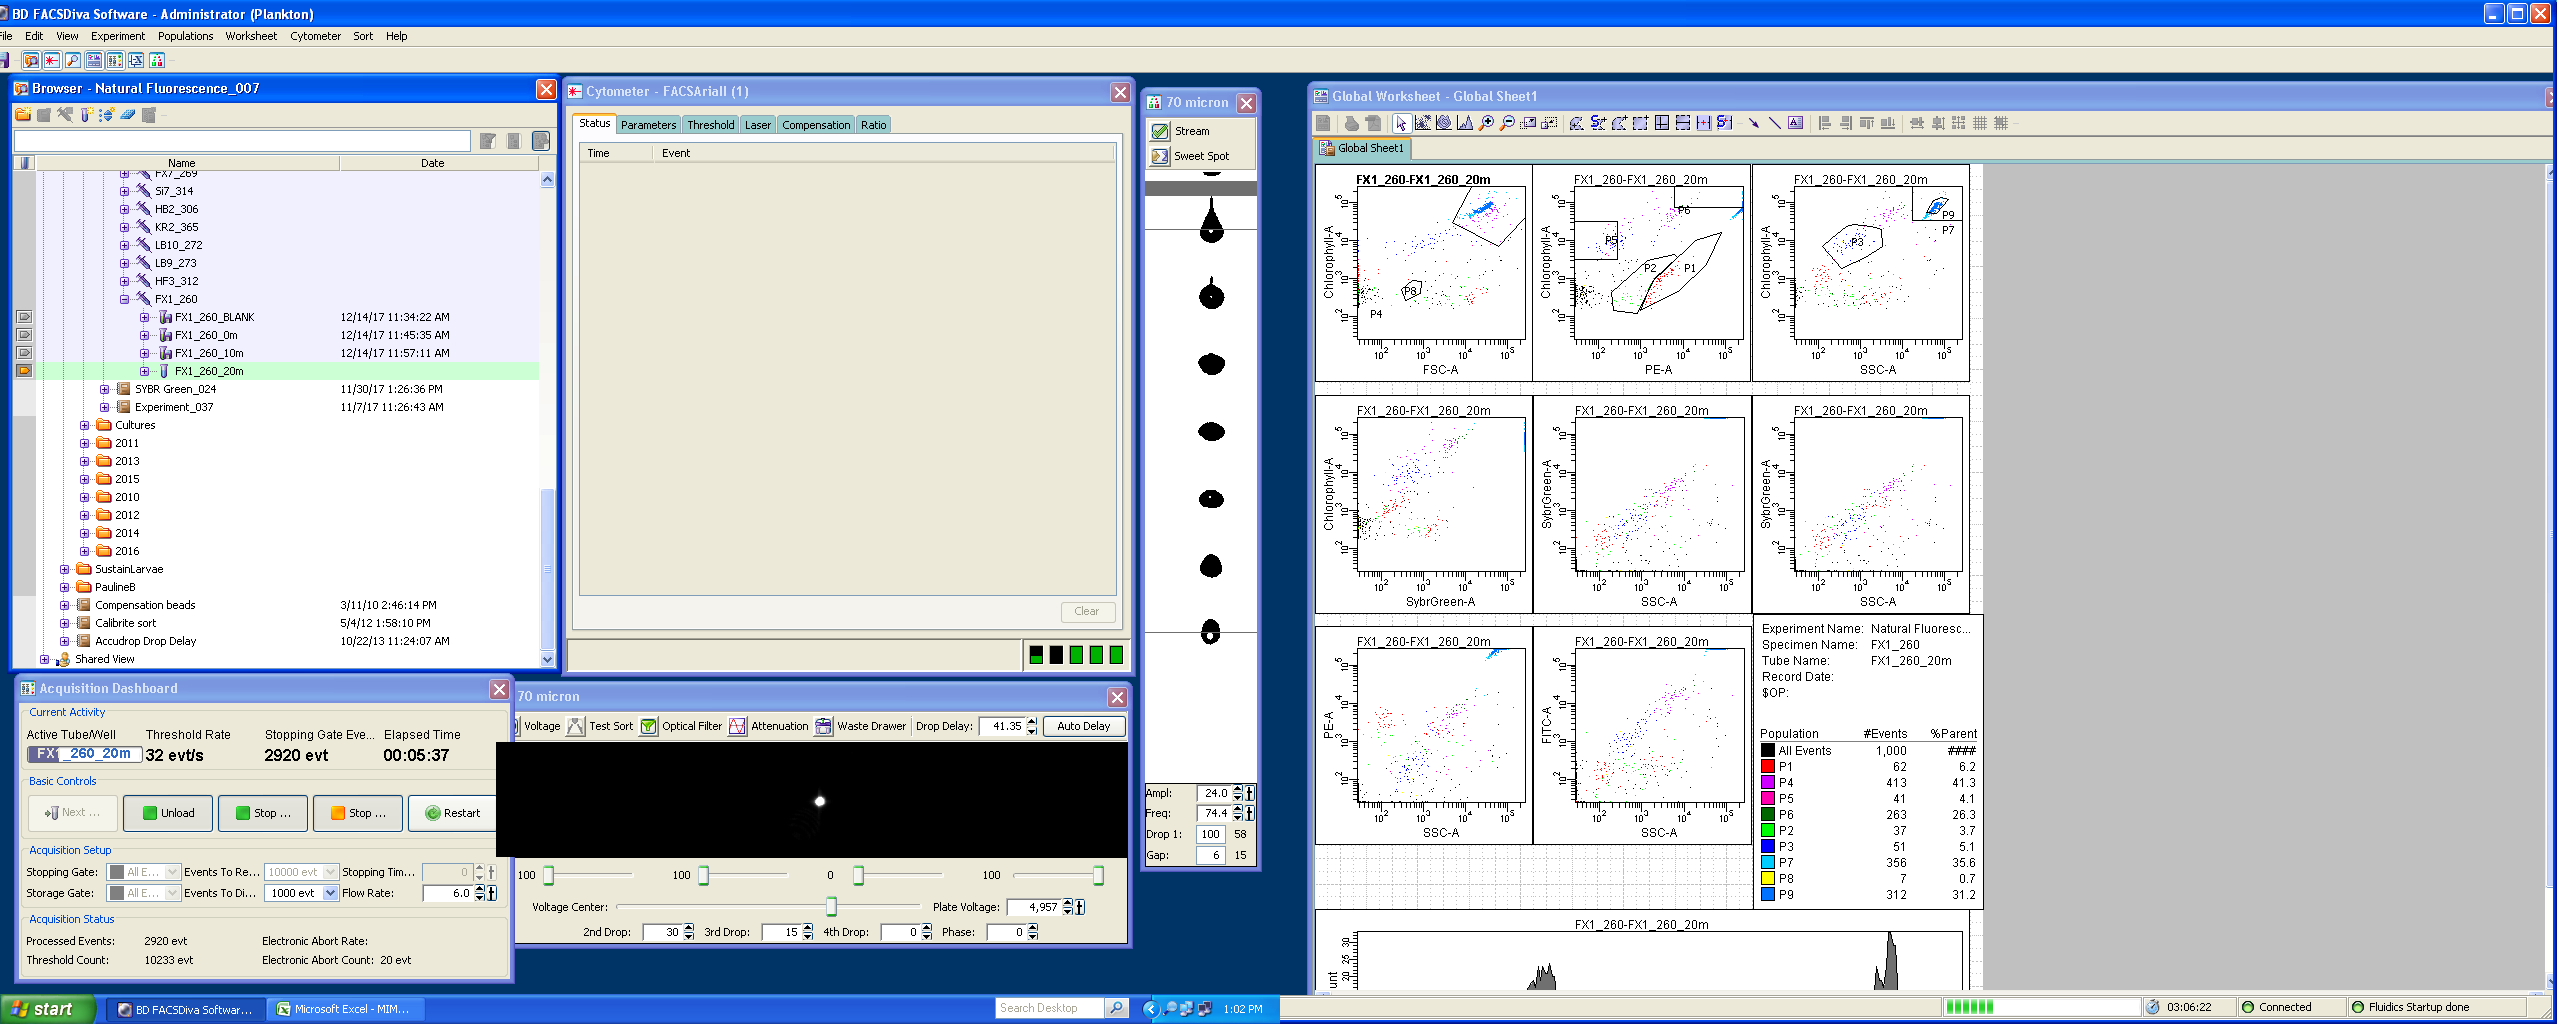
\includegraphics[width=\textwidth]{graphics/screenshots/20171214_bdfacsdiva.png}
% \end{figure}

% \begin{figure}[H] % position of the figure 
%     \centering
%     \caption{Global sheet for FX1 260 10m}
%     \label{fig:20171214_FX1_260_10m}
%     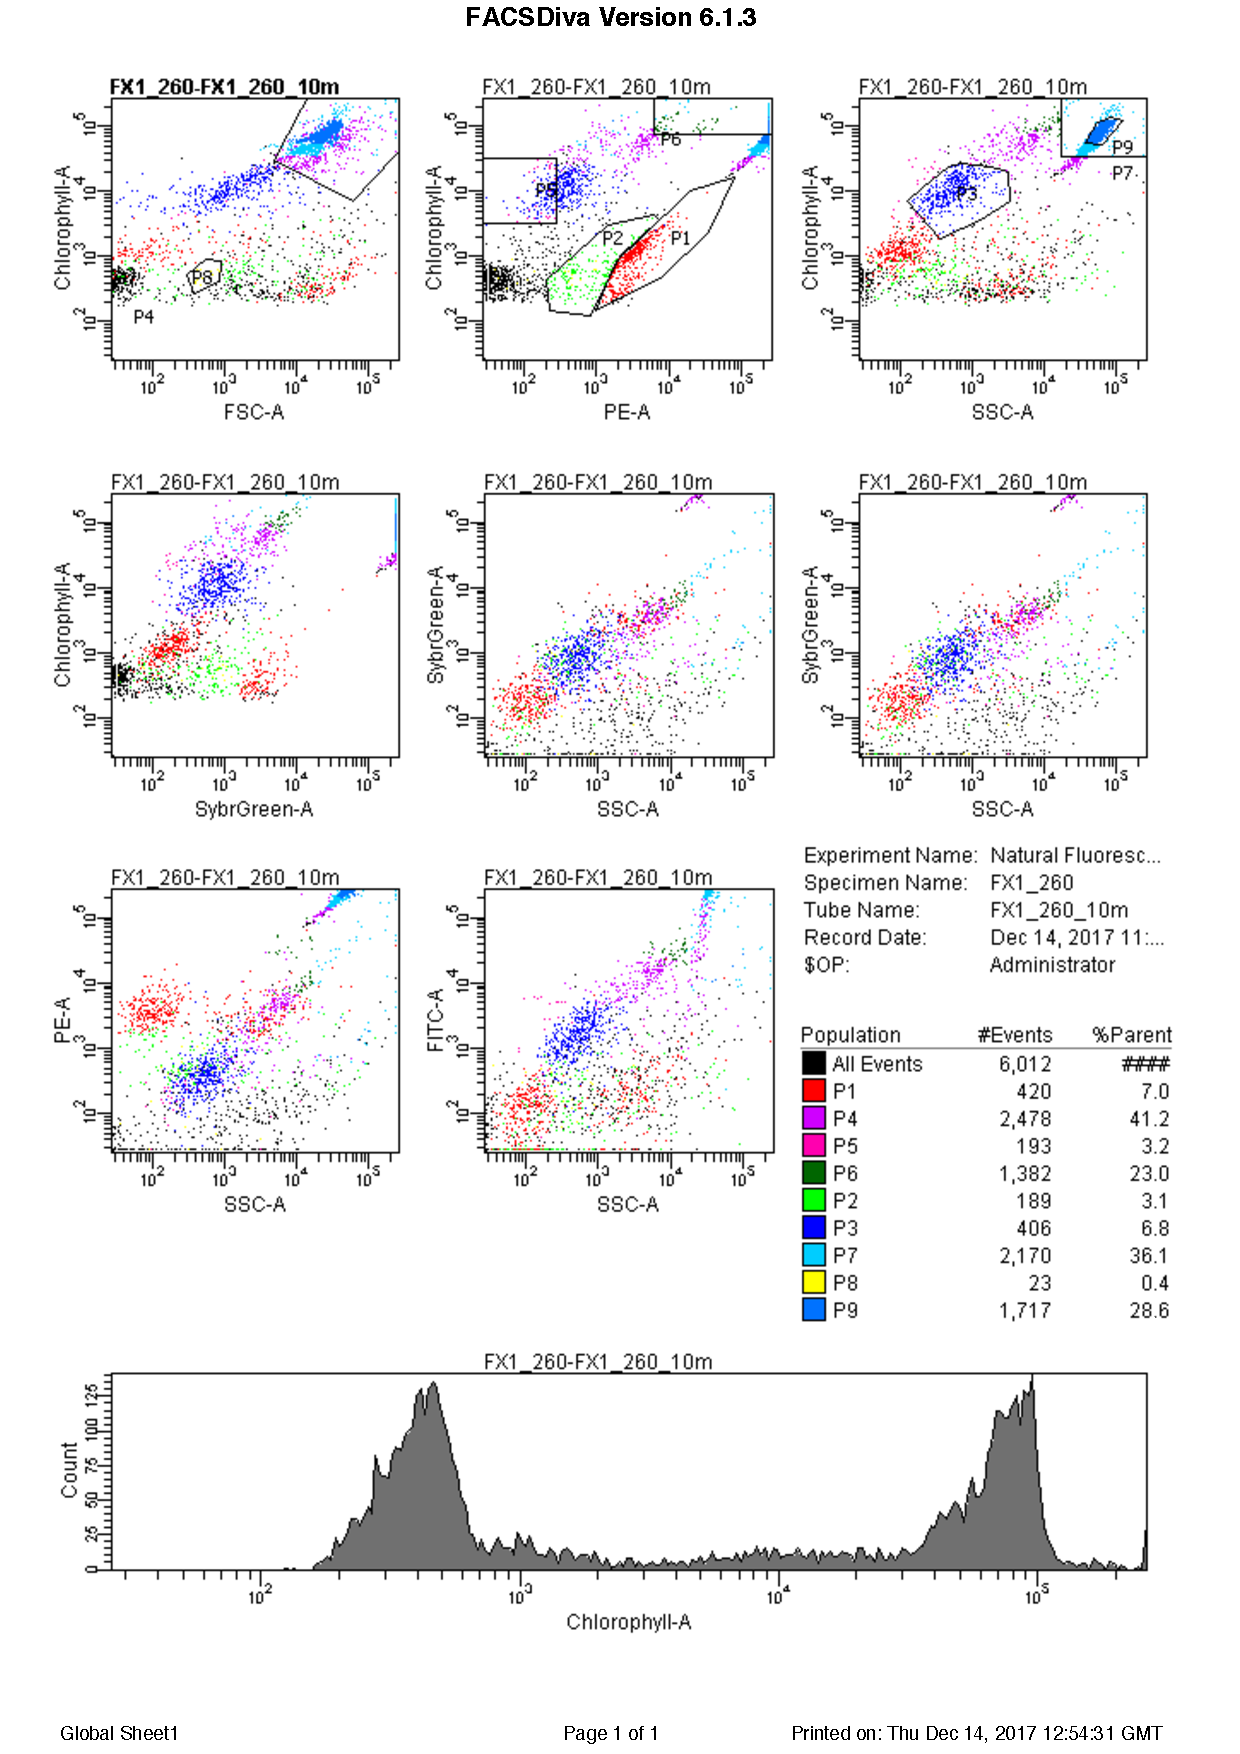
\includegraphics[width=\textwidth]{graphics/plots/20171214_FX1_260_10m.pdf}
% \end{figure}

\subsubsection{Analysis of stained samples}

\begin{enumerate}
\item Vortex SYBR Green working solution
\item Add 3~\textmu L of SYBR Green working solution into the 300~\textmu L of sea water sample
\item Vortex
\item Incubate in the dark at room temperature for at least 20 min (the analysis of the unstained samples can be done during this time).
\comment{I added the SYBR working solution at 12:30 AM.}
\item Vortex the working solution of beads
\item Add 3~\textmu L of beads to the sample (beads concentration in the sample is 1 in 100~\textmu L)
\item Vortex 
\item Open experiment on BD FACSDiva Software by double-clicking on "SYBR Green"
\item Follow the file creation and naming as described previously
\item Set up the flow rate to 1 (between 1 and 5 depending on the number of events)
\item Events per second should not be over 5000 - if the sample exceeds this, dilute in sterile water and re-run; note the dilution factor.
\item record the measurments for 2 min or until 10000 events have been counted (and try to reach 1000 beads to be statistically significant)
\end{enumerate}

\subsubsection{Flow cytometer shut-down}

\begin{enumerate}
\item Stop stream
\item Fill ethanol tank with water/ethanol (1/25)
\item Follow instructions on "Fluidics shut-down" and use water instead of cleaning solution prompted
\item Turm off flow cytometer (large gree buttom on the side of the machine)
\item Close pressure valve
\item Empty waste tank
\item Switch off computer
\item Record your name, number of hours spent of the flow cytometer and project number in the log book
\end{enumerate}

\comment{Towards the end of the day, I was getting very tired but I believe everything went well, even though I was processing samples until 7:00 PM.}